\section{General Notions of QEC}
It is sometimes said that the concept of quantum error correction is more remarkable than the concept of quantum computation itself \cite{girvin2019QECvideo}. Indeed, the fact that quantum error correction is in principle even possible is somewhat surprising, for three fundamental reasons: (1) the \textit{no-cloning} theorem \cite{ike-and-mike}, which forbids us from copying unknown quantum states to naively add redundancy; (2) the \textit{measurement problem}, also known as Born's rule, whereby measuring a quantum state causes it to collapse due to measurement backaction; and (3) errors on quantum states can be continuous-valued and are thus in some sense analog. Despite these somewhat severe restrictions imposed by quantum mechanics, quantum error correction (QEC) can still be realized --- and, in fact, has been done so.

In this thesis, we are concerned with a specific class of quantum error correcting codes called \textit{bosonic codes}, which store information in the continuous-variable degree of freedom of a quantum harmonic oscillator. Specifically, among the various bosonic codes that exist, we will focus on the so-called Gottesman-Kitaev-Preskill (GKP) grid code and its practical realization in experiment. In this chapter, we will introduce the basic notions of bosonic QEC and the GKP code, study specific theoretical proposals for error correction of the GKP codewords, and discuss various challenges and experimental considerations.


\subsection{Qubits and the Errors that Befall Them}






introduce qubit operators like $\sigma_z$ etc. since we'll use them throughout



\subsection{A Short History of QEC Codes}
Peter Shor etc etc etc. But also bosonic codes? Cite many papers here \todo{!}

\subsection{The Knill-Laflamme Condition for QEC}


\section{Overview of Bosonic Error Correction}
\subsection{Definitions and Notation \label{sec:2_BosonicQEC_Definitions}}
Here, we collect various definitions and identities from quantum optics that will be relevant to the discussion of bosonic QEC. Additional details can be found in Refs. \cite{shankar1994principles, raimond2006exploring, grynberg2010introduction}. We begin with an overview of the quantum harmonic oscillator, which is defined in terms of generalized position $\hat{x}$ and momentum $\hat{p}$ operators satisfying the commutation relation $[\hat{x}, \hat{p}] \equiv \hat{x}\hat{p} - \hat{p}\hat{x} = i\h$. The quantum Hamiltonian is given by
\begin{equation}
    \hat{H} = \frac{\hat{p}^2}{2m} + \frac{1}{2}m\omega^2 \hat{x}^2
\end{equation}
where $m$ denotes the mass and $\omega$ is the natural frequency \cite{shankar1994principles}. This is fully analogous to the classical Hamiltonian of a harmonic oscillator that we might study in a course on classical mechanics. In the quantum case, however, the oscillator will have quantized energy levels, which can be seen by introducing mode operators $\hat{a}, \hat{a}^\dagger$ that diagonalize the Hamiltonian:
\begin{align}
\begin{split}
     \hat{x} &= \sqrt{\frac{\h}{2m\omega}}(\hat{a} + \hat{a}^\dagger) \,\triangleq\, x_{\rm zpf} (\hat{a} + \hat{a}^\dagger) \\
     \hat{p} &= i\sqrt{\frac{m\h\omega}{2}}(\hat{a}^\dagger - \hat{a}) \,\triangleq\, \frac{i}{2x_{\rm zpf}} (\hat{a}^\dagger - \hat{a})
\end{split}
\end{align}
The commutation relation between $\hat{x}$ and $\hat{p}$ translates into an important relation: $[\hat{a}, \hat{a}^\dagger] = 1$. In quantum optics, it is also common convention to set $m, \omega, \h \to 1$, such that $x_{\rm zpf} \to 1/\sqrt{2}$. With these definitions in place, the oscillator Hamiltonian above takes on a simple form:
\begin{equation}
    \hat{H} = \h\omega\bigg(\hat{a}^\dagger\hat{a} + \frac{1}{2}\bigg) \,\triangleq\, \h\omega\bigg(\hat{n} + \frac{1}{2}\bigg)
\end{equation}
Here, we have defined the photon number operator $\hat{n} = \hat{a}^\dagger\hat{a}$ which tells us how many excitation quanta occupy an oscillator state. The energy eigenstates $\ket{n}$ (also known as \textit{Fock} states) satisfy $\hat{n}\ket{n} = n\ket{n}$, and thus the oscillator Hamiltonian satisfies $\hat{H}\ket{n} = E_n\ket{n}$ with energy levels $E_n = \h\omega(n + 1/2)$. The constant term $\h\omega/2$ is known as the zero-point energy; we mostly ignore it so that the oscillator Hamiltonian simplifies to just $\hat{H} = \h\omega \hat{a}^\dagger\hat{a}$. The mode operators $\hat{a}^\dagger, \hat{a}$ are referred to as \textit{creation} and \textit{anniliation} operators, since they act on Fock states via
\begin{equation}
    \hat{a}^\dagger\ket{n} = \sqrt{n+1}\ket{n+1}, \quad \hat{a}\ket{n} = \sqrt{n}\ket{n}.
\end{equation}
The Fock states $\{\ket{n}\}_{n=0}^\infty$ can be shown to form a basis for the formally infinite-dimensional Hilbert space $\mathcal{H}$ of a single oscillator mode; thus, $\ip{m}{n} = \delta_{n, m}$ and $\sum_n \op{n}{n} = \hat{I}$, where $\delta_{n, m}$ is the Kronecker delta and $\hat{I}$ is the identity operator on $\mathcal{H}$. 

In analogy with a classical oscillator, we can also define the \textit{position} and \textit{momentum} states of the quantum harmonic oscillator via the set of non-normalizable eigenstates $\ket{x}$ and $\ket{p}$, which satisfy $\hat{x}\ket{x} = x\ket{x}$ and $\hat{p}\ket{p} = p\ket{p}$ for $x, p \in \R$. These continuous-variable oscillator states satisfy
\begin{equation}
    \int_{x \in \R} \op{x}{x}dx = \int_{p \in \R} \op{p}{p} dp = \hat{I}
\end{equation}
and, like any conjugate pair of variables in quantum mechanics, can be related via Fourier transform: $\ket{x} = \frac{1}{\sqrt{2\pi}} \int_p dp e^{-ipq}\ket{p}$. One important set of identities the eigenstates $\ket{x}$ and $\ket{p}$ is the following: 
\begin{equation}
    e^{-iu\hat{p}}\ket{x} = \ket{x + u}, \quad e^{iv\hat{x}}\ket{p} = \ket{p+v}
\end{equation}
Effectively, the operators $\exp(-iu\hat{p})$ and $\exp(iv\hat{x})$ enable us to shift the position and momentum of the oscillator by $u$ and $v$ respectively. We can combine both into a quadrature displacement operator $\hat{D}(u, v) \equiv \exp(iv\hat{x} - iu\hat{p})$. Setting $\alpha = (u+iv)/\sqrt{2}$, we can then define the phase-space displacement operator $\hat{D}(\alpha) \equiv \hat{D}(u, v)$ as follows: 
\begin{equation}
    \hat{D}(\alpha) = \exp(\hat{a}^\dagger \alpha - \alpha^\ast \hat{a})
\end{equation}
Written in this canonical form, the displacement operator has several useful identities. In particular,  we have $\hat{D}^\dagger(\alpha) = \hat{D}(-\alpha)$ and $\hat{D}^\dagger(\alpha) \hat{a} \hat{D}(\alpha) = \hat{a} + \alpha$. The displacement operator also generates so-called \textit{coherent states} $\ket{\alpha} \equiv \hat{D}(\alpha)\ket{0}$ when operated on the vacuum state $\ket{0}$. These coherent states are eigenstates of $\hat{a}$, satisfying $\hat{a}\ket{\alpha} = \alpha\ket{\alpha}$, and can be explicitly constructed via:
\begin{equation}
    \ket{\alpha} = e^{-|\alpha|^2/2}\sum_{n=0}^\infty \frac{\alpha^n}{\sqrt{n!}} \ket{n}
\end{equation}

\noindent \textbf{Visualizing oscillator states.} In this section, we have introduced Fock states and coherent states as two important classes of oscillator states. For more general mixed states, we also typically represent oscillator states using a density matrix $\rho$. However, by far the most intuitive way to describe and visualize bosonic states is to use a phase-space quasiprobability distribution. One of the most common is the symmetric characteristic function $C(\beta)$, defined via: 
\begin{equation}
    C(\beta) = \ev{\hat{D}(\beta)} = \Tr[\rho \hat{D}(\beta)] 
\end{equation}
By taking the two-dimensional Fourier transform of this function in phase space, we arrive at the Wigner function
\begin{equation}
    W(\alpha) = \frac{1}{\pi^2}\int C(\beta) e^{\alpha\beta^\ast - \alpha^\ast\beta} d^2\beta
\end{equation}
By plotting $W(\alpha)$ as a function of $x = \sqrt{2}\mathrm{Re}(\alpha)$ and $p = \sqrt{2}\mathrm{Im}(\alpha)$, we can visualize an oscillator state $\rho$ in phase space. The Wigner function has some nice mathematical properties \todo{list the properties; also mention marginal distributions; }



\todo{Generate plot of Wigner/C for Fock states 0, 1, 2, 3, as well as a coherent state $\alpha$}

\subsection{Control, Nonlinearity, and Auxiliary Qubits}
\todo{a section about nonlinearity and drives? E.g. how an oscillator on its own can't do much, hence we need a nonlinear auxiliary element for control and measurement}

\subsection{Oscillator Error Mechanisms}

\todo{Introduce the master equation}


\section{A Brief Introduction to GKP Grid Codes}

The Gottesman-Kitaev-Preskill (GKP) grid code is a bosonic encoding that embeds a logical qubit nonlocally within the phase space of a harmonic oscillator. While the code itself has been known for two decades since the original proposal by Gottesman, Kitaev, and Preskill \cite{gottesman2001gkp} in 2001, it was only recently realized experimentally in trapped ions \cite{fluhmann2019gkp-expt, deneeve2022gkp-expt} and superconducting circuits \cite{campagne2020gkp-expt, sivak2023gkp-expt, nordquantique2023gkp-expt}. In this section, we will introduce the basic theory of the GKP code as well as its finite-energy counterpart, and then discuss the various components required for their experimental realization. 

\subsection{Ideal GKP Codes}
In general, GKP codes are defined by a lattice in the $(2N)$-dimensional phase space of $N$ quantum harmonic oscillators \cite{gottesman2001gkp, royer2022multimodegkp}. In this thesis, however, we will focus on the simplest case of a single oscillator ($N=1$) whose phase space is described by the quadrature coordinates $\hat{x}$ and $\hat{p}$ as discussed in Sec. \ref{sec:2_BosonicQEC_Definitions}. Following the original proposal of Gottesman, Kitaev, and Preskill, we can consider the square lattice with lattice constant $\ells = 2\sqrt{\pi}$ formed by the quadratures $\hat{x}$ and $\hat{p}$. The ideal GKP codewords associated with this lattice are defined as the simultaneous $+1$ eigenstates of the following two stabilizer operators: 
\begin{equation}
    \hat{S}_0^X = e^{-i\ells\hat{p}} = \hat{D}(\ell) , \qquad \hat{S}_0^Z = e^{i\ells\hat{x}} = \hat{D}(i\ell)
\end{equation}
where we define the reduced lattice constant $\ell = \ells/\sqrt{2}$ as the \textit{phase space} displacement associated with the quadrature displacement $\ell$. We can therefore write down the canonical GKP codewords directly. They are given by the $\hat{x}$ basis states
\begin{equation}
    \ket{0_L} \propto \sum_{j \in \Z} \ket{x = j\ells}, \qquad \ket{1_L} \propto \sum_{j \in \Z} \ket{x = (j + 1/2)\ells}.
    \label{eq:GKP_codewords_ideal}
\end{equation}
Together, these two codewords form a two-dimensional logical subspace $\mathcal{C} \equiv \{\ket{0_L}, \ket{1_L}\}$ within the infinite-dimensional Hilbert space $\mathcal{H}$ of the oscillator. We plot the wavefunctions for the codewords of Eq. \eqref{eq:GKP_codewords_ideal} in the position basis in Fig. \todo{make figure}, as well as the associated Wigner functions for the six cardinal states of the logical Bloch sphere: $\ket{\pm X_L}$, $\ket{\pm Y_L}$, and $\ket{\pm Z_L} \equiv \ket{0_L/1_L}$. By construction, we have $\hat{S}_0^X\ket{\mu_L} = \hat{S}_0^Z\ket{\mu_L} = \ket{\mu_L}$ for $\mu\in\{0, 1\}$, thus confirming that the operators $\hat{S}_0^X, \hat{S}_0^Z$ are indeed stabilizers. From Fig. \todo{make figure}, it is also clear that logical Pauli operators can be implemented via displacements of half the lattice constant: 
\begin{equation}
    \hat{X}_L^0 = \sqrt{\hat{S}_0^X} =  e^{-i\ells\hat{p}/2} , \qquad \hat{Z}_L^0 = \sqrt{\hat{S}_0^Z} = e^{i\ells\hat{x}/2}. 
\end{equation}

At this point, we might ask how the GKP states introduced above can be used for QEC. As originally proposed, the GKP code was designed to correct error channels that manifest as small phase space displacements of the oscillator, i.e. sending $(x, p) \to (x + \delta_x, p+\delta_p)$. The basic principle is as follows: observe that $[\hat{S}_0^Z, \hat{S}_0^X] = [e^{i\ells\hat{x}}, e^{-i\ells\hat{p}}] = 0$, i.e. the two GKP stabilizers commute and we can measure them simultaneously in their joint eigenbasis. This in turn implies that it is possible to measure $\hat{x}$ and $\hat{p}$ simultaneously as long as both are taken modulo $\ell/2$\footnote{Following \cite{royer2020gkp}, we will sometimes refer to the modular quadratures $\hat{x}_{[m]} \equiv \hat{x} \Mod m$ and $\hat{p}_{[m]} \equiv \hat{p} \Mod m$ with a symmetric modulo, i.e. $\hat{x}_{[m]}, \hat{p}_{[m]} \in [-m/2, m/2)$. We are specifically interested in $\hat{x}_{[\ells/2]}$ and $\hat{p}_{[\ells/2]}$.}. Therefore, if an error shifts the GKP grid $(x, p) \to (x + \delta_x, p+\delta_p)$, we can simply measure the modular quadratures and then apply a correction operation $\hat{D}(-\alpha)$ with $\alpha = (\delta_x + i\delta_p)/\sqrt{2}$ to re-center the grid. If the errors are small, i.e. $|\delta_x|, |\delta_p| < \ells / 4$, this results in a perfect recovery of the logical information, as depicted in Fig. \ref{fig:2-GKP-Ideal-QEC}(a). For realistic oscillators, most physical decoherence processes such as amplitude damping or dephasing occur via a continuous distortion of phase space, and can thus be corrected for if the GKP stabilizers are measured frequently enough \cite{gottesman2001gkp, glancy2006gkperror, albert2018performance-and-structure, noh2018performance-and-structure-pt2}. Among the various single-mode bosonic codes, it has been shown that the GKP code offers the best protection against photon loss, which is the dominant error mechanism for superconducting resonators \cite{albert2018performance-and-structure}. 
\begin{figure}[h]
    \centering
    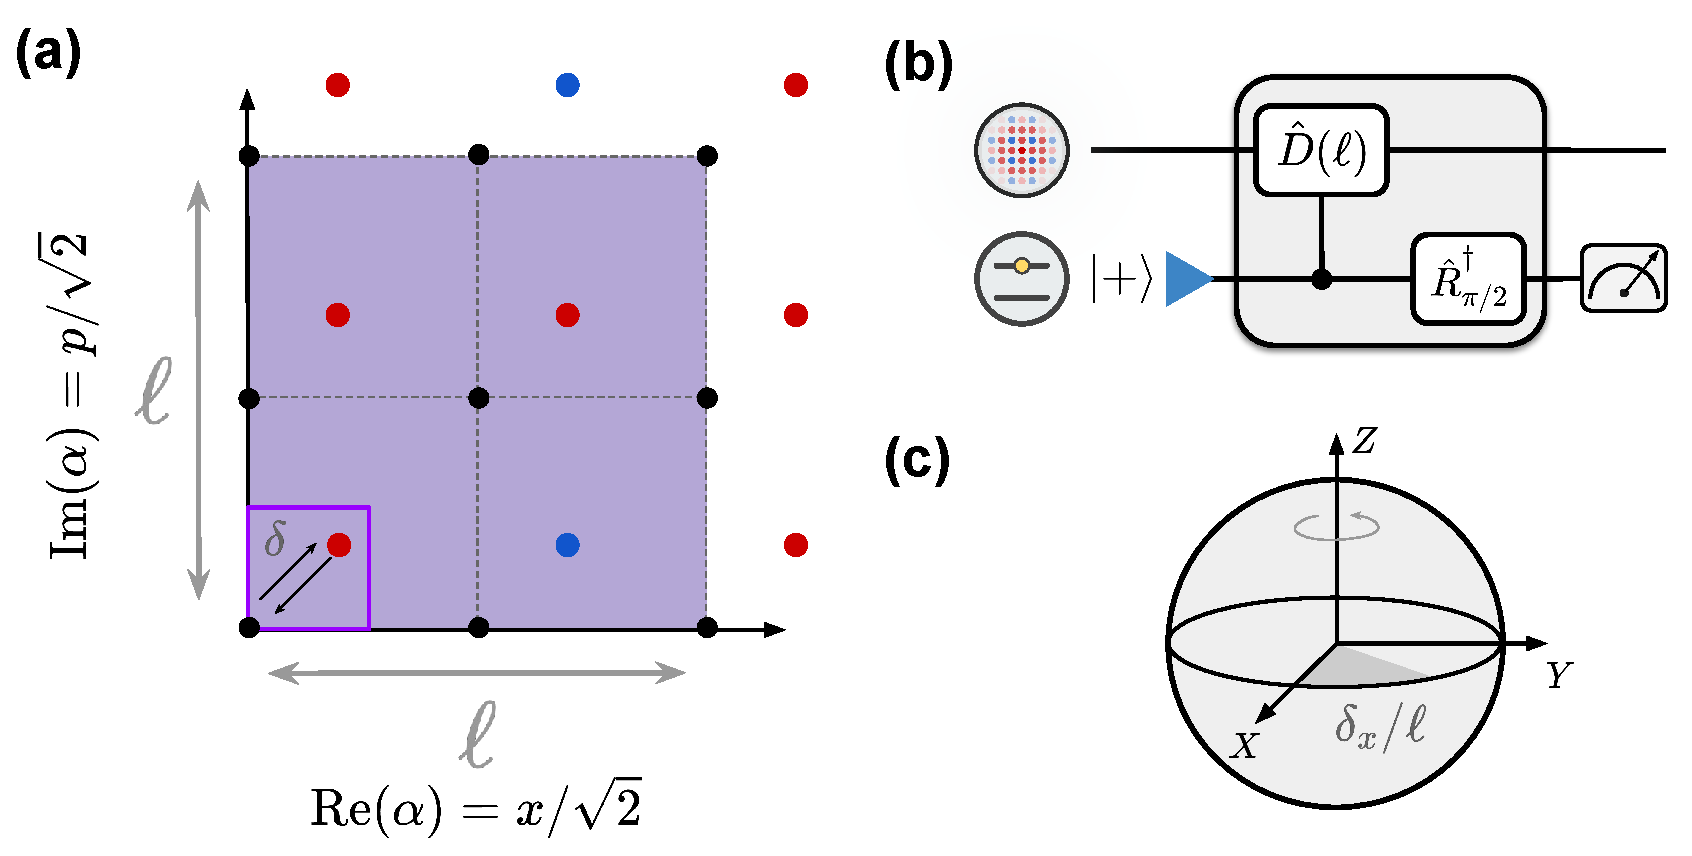
\includegraphics[width=\linewidth]{Figures/2/GKP Ideal QEC.pdf}
    \caption{\todo{caption}}
    \label{fig:2-GKP-Ideal-QEC}
\end{figure}

For an ideal GKP code, the actual stabilizer measurements can be carried out by using an auxiliary qubit as shown in Fig. \ref{fig:2-GKP-Ideal-QEC}(b). This circuit uses maps the stabilizer information onto the phase of the qubit using a conditional displacement operation
\begin{equation}
    {\rm CD}(\ell) = \hat{D}\bigg(\frac{\ell}{2}\bigg)\op{g}{g} + \hat{D}\bigg(\frac{-\ell}{2}\bigg)\op{e}{e} = \exp[\ell(\hat{a}^\dagger - \hat{a}) \sigmaz / 2].
\end{equation}
From the perspective of the oscillator, the CD gate implements a displacement conditioned on the state of the qubit; meanwhile, from the perspective of the qubit, this same operation can be seen as a rotation about the $z$-axis of the Bloch sphere by an amount $\ev{\hat{a}^\dagger - \hat{a}}\ell/2$



By measuring the qubit, one can then extract the error syndrome via a one-bit phase estimation \cite{terhal2016phase-estimation}. 


coupling the oscillator to an auxiliary qubit. 





$ $

\todo{How does GKP error correct? Measure stabilizers means measuring x and p mod l.}




\subsection{Finite-Energy GKP Codes}

While the ideal GKP codewords $\ket{\mu_L}$ make clear how the grid code can be used for error correction, it remains to be seen how to realize them in practice. On their own, the states $\ket{\mu_L}$ are non-normalizable superpositions of infinitely squeezed states that extend across the entire phase space of the oscillator. This presents two immediate problems: the first, perhaps most obviously, is that such infinite-energy states are not physical. The second, however, is that for realistic systems such as those we encounter in cQED, it is simply not feasible to have an arbitrarily large energy state in the oscillator. The reason for this is that the rates of various physical error channels scale with the number of photons/excitations. For example, amplitude damping where the photon loss rate $\Gamma_n$ with which the Fock state $\ket{n}$ decays to $\ket{n-1}$ scales as $\Gamma_n = n\Gamma_1$, where $\Gamma_1$ is the single-photon loss rate. Another example is the self-Kerr nonlinearity that a resonator inherits from its coupling to any nonlinear auxiliary control element (cf. Chapter \ref{ch:3_cQED}). 

To remedy the situation above, it is necessary to bound the squeezing of the GKP states and limit their extent in phase space. Furthermore, one must design error correction strategies that maintain the oscillator photon number so that such errors do not accumulate over time \cite{campagne2020gkp-expt}. We can realize physical, finite-energy GKP states by applying an envelope operator $\hat{E}_\Delta$ to the codewords \cite{royer2020gkp}. A natural choice is a Gaussian envelope $\hat{E}_\Delta = \exp(-\Delta^2 \hat{a}^\dagger\hat{a})$, which gives the individual peaks of the GKP states a finite width $\Delta$ while also applying an overall Gaussian envelope of width $1/\Delta$ to the entire grid. We define the finite-energy GKP codewords as 
\begin{equation}
    \ket{\tilde{\mu}_L} = \mathcal{N}_\Delta \hat{E}_\Delta \ket{\mu_L}
\end{equation}
for $\mu \in \{0, 1\}$, where $\mathcal{N}_\Delta$ is a normalization factor. These approximate GKP states $\ket{\tilde{\mu}_L}$ are non-orthogonal for non-zero $\Delta$, and are also no longer eigenstates of the ideal stabilizers $\hat{S}_0^{X/Z}$. However, it turns out that it is still possible to define exact stabilizers for the finite-energy code
\begin{equation}
    \hat{S}_\Delta^{X/Z} = \hat{E}_\Delta\,\hat{S}_0^{X/Z}\,\hat{E}_\Delta^{-1}
\end{equation}
which, by construction, satisfy $\hat{S}_\Delta^{X/Z}\ket{\tilde{\mu}_L} = \ket{\tilde{\mu}_L}$. We can similarly define regularized logical Pauli operators $\hat{X}_L^\Delta = \hat{E}_\Delta \hat{X}_L^0 \hat{E}_\Delta^{-1}$ and $\hat{Z}_L^\Delta = \hat{E}_\Delta \hat{Z}_L^0 \hat{E}_\Delta^{-1}$ via the same transformation. Clearly, as $\Delta \to 0$, the finite-energy GKP states and operators will approach their ideal infinite-energy counterparts, albeit at the expense of a higher average photon number in the codewords 
\begin{equation}
    \bar{n}_{\rm GKP} = \frac{1}{2} \sum_{\mu\in \{0,1\}} \mel{\tilde{\mu}_L}{\hat{a}^\dagger\hat{a}}{\tilde{\mu}_L} \approx \frac{1}{2\Delta^2} - \frac{1}{2}
\end{equation}
and the detrimental effects that come with it. Conversely, increasing $\Delta$ too much results in a non-negligible loss in fidelity due to the increasing finite overlap $\ip{\tilde{0}_L}{\tilde{1}_L}$, and in general reduces the code's ability to correct errors \cite{royer2020gkp}. We can therefore view $\Delta$ as a controllable parameter which determines the `size' of the GKP code, and whose value can be optimized in experiment. 


\section{Open-Loop GKP Error Correction}

In circuit QED, there are various approach one could take to simply \textit{prepare} GKP states, e.g. via optimal control protocols such as GRAPE \cite{khaneja2005grape, reinhold2019thesis}, SNAP \cite{krastanov2015-SNAP, heeres2015-SNAP, fosel2020-SNAP}, or ECD \cite{eickbusch2022-ECD}; via periodic (Floquet) driving in a SQUID \cite{gkp-periodic-drive2024}; or by engineering superconducting circuits with GKP-like ground states \cite{rymarz2021hardwaregkp}. However, we are generally more interested in protocols that prepare \textit{and} continuously stabilize GKP states via stabilizer measurements and active error correction. For ideal GKP codewords, we saw how to do this with phase estimation in Fig. \ref{fig:2-GKP-Ideal-QEC}. On the other hand, for realistic GKP codewords in practice, we need to measure the corresponding stabilizers $\hat{S}_\Delta^{X/Z}$ instead. It turns that this is possible to do by modifying the circuit in Fig. \ref{fig:2-GKP-Ideal-QEC} to account for the finite-energy envelope \cite{fluhmann2019gkp-expt, campagne2020gkp-expt, royer2020gkp, deneeve2022gkp-expt}; furthermore, QEC can be realized ``autonomously'' by replacing the measurement-based feedback step with an unconditional qubit reset. More precisely, we refer to this as \textit{open-loop} error correction (in the language of control theory) to distinguish it from QEC based on feedback control.

To arrive at the result above, it ends up being helpful to take a different view of the QEC process as a form of engineered dissipation \cite{royer2020gkp, vlad2023thesis}. In this picture, errors can be described by excitations out of the GKP code manifold and error correction involves realizing a dissipative quantum channel to `cool' these excitations and stabilize the code space. Following the theoretical treatment in Ref. \cite{royer2020gkp}, the general dissipation channel on the oscillator can be mapped to an interaction between the oscillator and an auxiliary qubit that is reset, i.e. effectively transferring entropy out of the system. We refer the reader to Refs. \cite{royer2020gkp, sivak2023gkp-expt, vlad2023thesis} for a rigorous derivation and discussion of this theory\footnote{We also point out Refs. \cite{sellem2023gkp, sellem2024gkp} which introduce an entirely different dissipation channel for the GKP code, though the main idea there is also to autonomously stabilize the code space albeit with more dissipators.}, and here instead just convey the main result. Based on different Trotter decompositions of the generalized dissipation channel in \cite{royer2020gkp}, there are actually several candidate qubit-oscillator circuits/protocols that can realize open-loop QEC of the finite-energy GKP code. In this thesis, we work primarily with the Small-Big-Small (SBS) protocol\footnote{The other two protocols are called Sharpen-Trim (ST) and Big-Small-Big (BSB). Both require two large CD gates, and ST also has two reset steps. Meanwhile SBS requires just one of each (see next section).}, shown below. 
\begin{figure}[h]
    \centering
    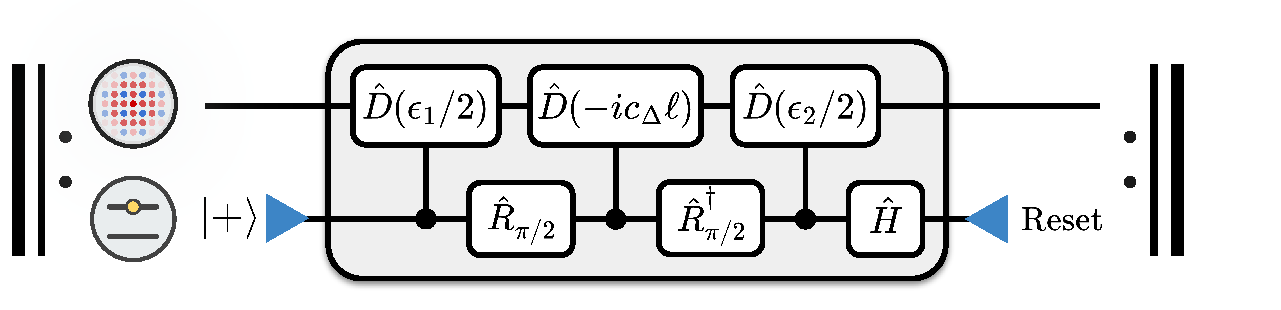
\includegraphics[width=0.85\linewidth]{Figures/2/SBS.pdf}
    \caption{Caption. In certain cases, the final Hadamard can be discarded and absorbed into reset.}
    \label{fig:2-SBS}
\end{figure}

\subsection{The Small-Big-Small (SBS) Protocol}
\textbf{Overview.} The SBS circuit consists of three conditional displacement gates interleaved by qubit rotations. The middle CD involves a large phase space displacement of magnitude $c_\Delta \ell \approx \ell$, and it effectively realizes phase estimation to measure the GKP stabilizer. Here we have defined $c_\Delta \equiv \cosh(\Delta^2)$, and note that $c_\Delta \approx 1$ for all practical values ($\Delta \lesssim 0.4$) of the GKP size. Meanwhile, the first and last CD operations are smaller corrections that account for the finite-energy envelope and perform autonomous error correction respectively (see e.g. \href{https://youtu.be/TOQzHkgsH_E?t=1045}{this talk}). From theory, we have $\epsilon_1 = s_\Delta \ell$ with $s_\Delta \equiv \sinh(\Delta^2) \approx \Delta^2$, and we nominally expect $\epsilon_2 = \epsilon_1$. However, in Ref. \cite{sivak2023gkp-expt}, the authors optimized the two small displacements independently and found, through use of a reinforcement learning agent, that choosing $\epsilon_2 \gtrsim \epsilon_1$ gave the best QEC performance. This observation has since been corroborated in simulation when accounting for all error channels acting during the SBS unitary, and was also reported in another experiment \cite{nordquantique2023gkp-expt}. Essentially, although $\epsilon_1 = \epsilon_2$ holds for a lossless circuit, when including loss the optimal ratio $\epsilon_2/\epsilon_1$ turns out to be strongly dependent on the actual error channels involved, and is thus another free parameter (like $\Delta$) that can be tweaked in experiment to get the best QEC gain. Finally, it is important to note that the circuit above carries out phase estimation for the $\hat{S}_\Delta^{Z}$ stabilizer; to get the circuit for the $\hat{S}_\Delta^{X}$ stabilizer, we just map ${\rm CD}(\beta) \to {\rm CD}(i\beta)$. The full QEC sequence for SBS then involves alternating between the two circuits to stabilize both quadratures. 

\noindent \textbf{Kraus Operators for SBS.} We can describe the SBS protocol in a more quantitative manner by considering it as a quantum channel. To this end, let us imagine that the SBS reset step is implemented via a measurement-based active reset. In this case, although the oscillator QEC is still `autonomous', we would have access to the error syndromes by looking at the measurement statistics of the qubit. A subtle yet interesting feature of the circuit above is that---in the absence of errors---it leaves the qubit and oscillator completely disentangled after the unitary evolution (gray box in Fig. \ref{fig:2-SBS}). Thus, if no error occurs, the qubit state will end up in $\ket{g}$ before reset. In our current measurement-based reset approach, then, a measurement outcome $\ket{g}$ would signify ``no error'' while a measurement outcome $\ket{e}$ would imply that an error was detected and corrected. Based on these two outcomes, we can write down the action of the SBS circuit above on just the oscillator state using a pair of Kraus operators $\hat{K}_g^Z, \hat{K}_e^Z$, which are given by\footnote{I owe a huge thanks to Jonathan Pelletier for his help deriving these expressions for the general case $\epsilon_1 \neq \epsilon_2$.}:     
\begin{align}
    \begin{split}
        \hat{K}_g^Z &= \cos\bigg(\frac{\epsilon_2 \sqrt{\pi}}{2\sqrt{2}}\bigg)\Bigg[\cos\bigg(\frac{\epsilon_2 + \epsilon_1}{2\sqrt{2}} \hat{p}\bigg)\cos(\sqrt{\pi} \hat{x}) + i\sin\bigg(\frac{\epsilon_2 - \epsilon_1}{2\sqrt{2}} \hat{p}\bigg)\sin(\sqrt{\pi} \hat{x})\Bigg] \\
        &\quad + \sin\bigg(\frac{\epsilon_2 \sqrt{\pi}}{2\sqrt{2}}\bigg)\Bigg[\cos\bigg(\frac{\epsilon_2 - \epsilon_1}{2\sqrt{2}} \hat{p}\bigg)\cos(\sqrt{\pi} \hat{x}) - i\sin\bigg(\frac{\epsilon_2 + \epsilon_1}{2\sqrt{2}} \hat{p}\bigg)\sin(\sqrt{\pi} \hat{x})\Bigg]
    \end{split} \\
    \begin{split}
        \hat{K}_e^Z &= -\cos\bigg(\frac{\epsilon_2 \sqrt{\pi}}{2\sqrt{2}}\bigg)\Bigg[i\sin\bigg(\frac{\epsilon_2 + \epsilon_1}{2\sqrt{2}} \hat{p}\bigg)\cos(\sqrt{\pi} \hat{x}) + \cos\bigg(\frac{\epsilon_2 - \epsilon_1}{2\sqrt{2}} \hat{p}\bigg)\sin(\sqrt{\pi} \hat{x})\Bigg] \\
        &\quad -\sin\bigg(\frac{\epsilon_2 \sqrt{\pi}}{2\sqrt{2}}\bigg)\Bigg[i\sin\bigg(\frac{\epsilon_2 - \epsilon_1}{2\sqrt{2}} \hat{p}\bigg)\cos(\sqrt{\pi} \hat{x}) - \cos\bigg(\frac{\epsilon_2 + \epsilon_1}{2\sqrt{2}} \hat{p}\bigg)\sin(\sqrt{\pi} \hat{x})\Bigg]
    \end{split}
\end{align}
For an input state $\hat{\rho}\otimes \op{+}{+}$ to the SBS circuit, the oscillator state $\hat{\rho}$ after unitary evolution and reset is given by
\begin{equation}
    \hat{\rho} \mapsto \mathcal{R}_\Delta^Z(\hat{\rho}) = \hat{K}_g^Z \hat{\rho} \hat{K}_g^Z{}^\dagger + \hat{K}_e^Z \hat{\rho} \hat{K}_e^Z{}^\dagger  
\end{equation}
where $\mathcal{R}_\Delta^Z$ is the rank-2 dissipator towards the $+1$ eigenspace of $\hat{S}_\Delta^Z$. To get the equivalent dissipator $\mathcal{R}_\Delta^X$ for the stabilizer $\hat{S}_\Delta^X$, we can map $\hat{K}_{g/e}^Z \to \hat{K}_{g/e}^X$ by making the replacement $(x, p) \to (p, -x)$. Finally, the quantum channel for the full SBS QEC cycle is $\mathcal{R}_\Delta = \mathcal{R}_\Delta^X \circ \mathcal{R}_\Delta^Z$. 

In practice, we envision in our experiments using a fully unconditional qubit reset rather than measurement-based feedback. In this case, we won't have access to the measurement statistics (as the protocol will be truly \textit{open-loop}), and the final qubit Hadamard gate can also be omitted from the protocol. However, for theoretical analysis and certain numerical simulations, it makes things considerably easier to continue working in the artificial measurement-based feedback picture using the Kraus operators for SBS.

\noindent\textbf{Logical Pauli Measurements.} In addition to stabilizer measurements, we will also want to 




\subsection{Simulations with SBS: I. Oscillator Error Channels}

\subsection{Simulations with SBS: II. Control Qubit Error Channels}













\section{Experimental Considerations}

\subsection{Qubit-Oscillator Coupling}

\subsection{Realizing Conditional Displacement Gates}

\subsection{Simulations with SBS: III. Kerr and Dispersive Shift}

